\chapter{Search by Face Similarity}
\label{ch:face_search}

In this chapter, we propose another approach to the \acrshort{cbir} task. This approach focuses only on the case, where the images include people.
We investigate the option of finding the target image based on the person's face in the image and other faces in the dataset.

This approach arises from practical reasons. Once we investigated the V3C1 dataset, we realized that in many of the images are people. We can use the previously investigated approaches based on the location and visual similarity to find the target image. However, with the increasing number of images showing people, it becomes difficult to retrieve the correct target image. Simply searching for a person in the top left corner would retrieve all images with a person in the said corner (not just the one we are looking for). Also, finding a good representative face with similar background becomes a challenging task.

In this chapter, we aim to provide a search mechanism employing finer features of one's face. We provide a simple search structure to investigate the faces in the dataset.

We first extract the faces from the dataset, and then we obtain a descriptor for each one of them. Based on these descriptors, we organize the faces into a traversal structure supporting navigational commands.

The task of comparing faces of the people and saying which look more similar has its roots in the human perception of faces. Therefore, to evaluate the individual steps, we conduct experiments with human subjects.

Our experiments suggest that the feature space of the descriptors has a limited power to sort people based on the similarity in a way people do. Based on that, we implement the traversal structure, which can be used with the presented descriptors or any other descriptors of the faces that could be developed in the future.


\section{Overview}

Our goal is to propose a traversal structure based on the faces found in the dataset. Ideally, we would like to group similar faces so that users can quickly decide if the group of people corresponds to the target face they look for, or not.

% We, as people, do not perceive the similarity of faces always the same way. We hypothesize that when we two people find the most similar faces to a given face, they will not choose the same set. We verify this hypothesis in the case study, presented in section \ref{s:case_study}.

The question we ask in the following sections is if the face descriptors can sort people based on the similarity, similarly to human perception. If yes, then we can argue that traversal structure based on these face descriptors may help. We leave experiments with additional descriptors for future work. In our case, we compare only one type of face descriptors to human perception, although, in future work, it may be experimented further with other descriptors.

% If we do not observe any correlation between the ordering based on the descriptors and survey responses, then the descriptors would not be able to group similar faces as people do.

\section{Extraction of the faces}

If we look at the dataset, we notice that only a small portion of the people look directly into the camera. Since the images come from the videos, most of the people captured are doing some activity and not looking directly into the camera. As discussed in section \ref{s:dlib}, we select the CNN based approach to extract the faces since it worked better with a wider variety of poses.

For our experiment, we use only a part of the original dataset. We extract faces only from the first 316 videos of the V3C1 dataset. Again, we firstly use image extraction from videos (refer to section \ref{s:dataset}), and only then we extract faces from images. 

From these 316 videos, we were able to extract more than seventeen thousand faces. However, after investigation of the dataset, we found out that many of the extracted faces had too low resolution. The majority of the extracted faces did not even cover 5\% of the image. Therefore, we decided to filter out the dataset further and remove all the faces that did not cover at least ten percent of the image. The distribution of the area covered by a face is displayed in figure \ref{fig:faces_size_distribution}. After the filtering,  we obtained 2047 faces from the 316 videos. A random selection of faces is shown in figure \ref{fig:random_selection_faces}. 

We then visually investigated the extracted faces. The dataset contains people of different ethnicity, age, and gender. The faces are displayed from a wide range of angles, including even full side views. Some of the people wear glasses, headphones or other accessories. The dataset also contains some pictures of children. The model also extracted a few drawn faces or faces of sculptures.

% Because most of the faces cover at least 5\% of the image, we decided to filter out too small faces. We filtered out the faces, which covered less than ten percent of the image.

\begin{figure}
    \centering
    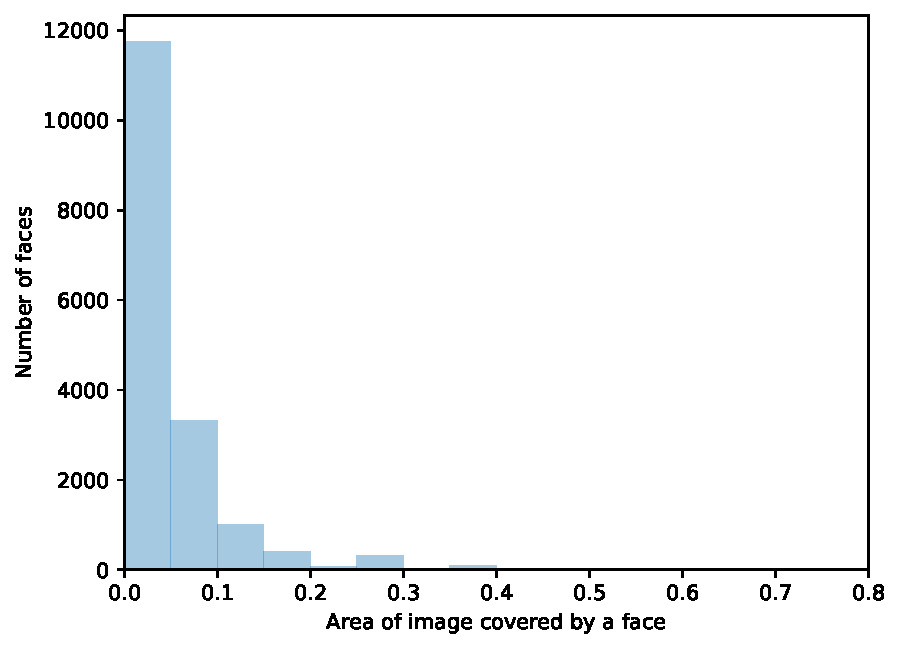
\includegraphics[width=0.7\linewidth]{graphs/faces_size_distribution.pdf}
    \caption{Area of image covered by a face}
    \label{fig:faces_size_distribution}
\end{figure}

\begin{figure}
    \centering
    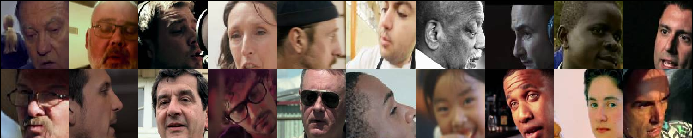
\includegraphics[width=0.98\linewidth]{img/random_selection_faces.pdf}
    \caption{A random selection of faces extracted from the dataset.}
    \label{fig:random_selection_faces}
\end{figure}

\section{Face similarity based on the deep features}

For extracting descriptors (i.e., feature vectors), we use the dlib pre-trained model, as discussed in \ref{s:dlib}. The network outputs vectors from space $\mathbb{R}^{128}$. We use the output of the network directly as our feature vectors. 

Note that often \emph{face features} refer to the specifics of the face landmarks, the color of the eyes, size of the lips, etc. To avoid confusion, we use the term \emph{face encoding} or descriptors for feature vectors obtained by the neural network. Such face encodings are usually from the space $\mathbb{R}^n$, in our case $n=128$.

After obtaining the face encodings for our dataset of 2047 faces, we were interested in if this feature space, created by the \acrshort{cnn} is able to sort the faces based on the similarity in a way people do. 

The library, from which we use the model, refers to a threshold 0.6 in the euclidean distance as the threshold with the highest accuracy on the verification task. The example of the closest faces based on this threshold is displayed in figure \ref{fig:closest_faces}. The top left image belongs to the target face. In the provided example, we can see that the face encodings close to our target face truly belong to the same person. Unfortunately, we can see, that with increasing distance other people appear even below the threshold 0.6.


\begin{figure}
    \centering
    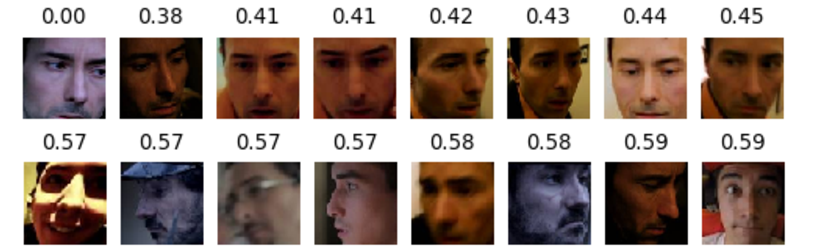
\includegraphics[width=\linewidth]{img/man_closest_faces.pdf}
    \caption{Examples of the retrieved closest faces to the target face (top left) based on euclidean distance. The number above each image represents the distance from the target.}
    \label{fig:closest_faces}
\end{figure}

\section{Case study}
\label{s:case_study}

% We want to find out if the space of the obtained face features, can order faces based on their similarity similarly to human subjects.

In this section, we investigate a possible correlation between the given faces as perceived by humans and the distances between their encodings.

We conducted a study with 25 participants. We presented to them a $10\times10$ grid of randomly selected faces from the dataset. 
Then we showed them ten randomly selected target faces of different people (same set of faces to each participant). We asked the participant to select for each target face \emph{exactly} three faces from the grid that looked the most similar. 

%Then we asked them to select exactly three faces, which are the most similar to the provided target face. Our test contained ten randomly pre-selected faces of different people. Out of 10, one of them was a child, we estimate below ten years old. Two of the other target faces were present in the grid.

Out of 10 target faces, three were also represented in the grid. Two of the faces were extracted from the same image, i.e., the same angle of the face. The third face, which was also present in the grid, had two representants in the grid. First identical to the target face and the second with only a minor change of the angle.

Firstly, we investigate how likely it is that the human subject notices that the face they are looking for is also present in the grid. In the first case, twenty-four out of 25 respondents selected the face corresponding to the same target person. In the second case, only 20 respondents found the face in the grid. We assume that the first case was ``easier'' because the face comes from black and white image, therefore, was easier to notice. In the third case, two face views of the target person were available in the grid. Nine respondents selected both correctly, and eleven respondents selected only one of them. 

As our next step, we empirically evaluate, if the model used for obtaining the face encodings, can sort the faces based on the distances similarly as human subjects do.

We further investigate the seven target faces, which were not present in the grid. Excluding the three cases, where the target face is in the grid, we avoid overestimating the quality of our model, since we know, that the model is performing well on the verification task. For each of the faces $F\in G$ from the grid $G$, we compute the euclidean distance from the target face $T\in D$, where $D$ denotes our dataset of faces (between their encodings). We then reorder the faces from the grid based on this distance (similar to the ranking from the previous chapters). 

Formally we define distance $\gamma$ between faces $F, F' \in D$ based on the descriptor extraction function $f$ and euclidean distance $d_e$:

$$
\gamma(F, F') = d_e(f(F), f(F'))
$$

This definition allows us to rank faces in the grid $G$ based on the target face $T$:

$$
    r_T(F) = |\{F'\in G\mid\gamma(F', T) < \gamma(F, T)\}|
$$

Again, to ``break ties'', we use any arbitrary total ordering $<_F$ over faces, as in \autoref{s:task_formulation}.

% \todo{chyba kucerava zatvorka}
% $$
%  r_T(F) = |\{F'\in G\}| \gamma(F', T) < \gamma(F, T) \lor (\gamma(F', T) = \gamma(F, T) \land F' <_F F)\} |
% $$

% The closest face has the lowest index. We refer to the face's index in the sorted set of faces as $rank_t$ with respect to the target face $t$.

Note that this ranking function is a bijection between the faces in the grid and a set $\{0, 1, \ldots |G| - 1\}$, given the target image. Therefore, it is reversible, i.e., we can obtain the face from the given rank. Based on this ranking, and the data obtained from the respondents, we aim to verify the correspondence of the ranking based on distances of the encodings and the most similar faces as identified by the respondents.

This allows estimation (based on the results of the survey)  of the probability $p$ that for given target face $T$ user selects a face with rank $R$. We also denote the number of respondents that selected face $F$ for target face $T$ as $N_T(F)$. The resulting probability then is:

$$
    p_T(R) = \frac{N_T(r_T^{-1}(R))}{25}
$$

Finally, to provide comprehensive overview, we compute combined probability of selecting face with rank $R$ by combining the results for all target faces $\mathcal{T}$:

$$
p(R) = \frac{\sum_{T\in \mathcal{T}} p_T(R)}{|\mathcal{T}|}
$$

Note that as each user selects three faces, it holds: $\sum_{R\in\{0,1,\ldots99\}} p(R) = 3$.

We plot the empirical probability $p$, of a user selecting the face on the $k$-th rank, given the target face. If the user is fully coherent with the model, they would choose the closest three faces based on the euclidean distance, and for the $R \in \{0,1,2\}$ we would see a probability $p(R) = 1$ and zero otherwise. 

This plot of the probabilities is displayed in figure \ref{fig:survey_distribution}. Note that, this is not a probabilistic distribution, since it does not sum up to one, but rather three. We do not normalize this plot, so we can talk about the probability, given our experimental settings, i.e., selecting exactly three faces.

% In the same figure \ref{fig:survey_distribution} we can see the distribution only of the seven presented faces.

% In this experiment we excluded a target face, which belonged to a child (the only child among the 10 target faces). \todo{}.

We are interested in the distribution of ranks given the faces selected by the users. We want to know if there is any correlation between similarity in the feature space and the similarity perceived by the human respondents. 

% From the survey responses we create a heatmap for each task. The size of the heatmap corresponds to the size of the face grid, i.e., $10\times10$. The element on the position $task, i, j$ of the heatmap corresponds to the number of times, the face at $i$-th row and in $j$-th column was selected in the given $task$. We use the heatmap and the ranking based on the distances in the feature space, to compute, how many closest faces from feature space were actually selected. We do the same for each rank. The normalized results over all possible ranks (from 0 to 99) are plotted in the figure \ref{fig:survey_distribution}. If the users perception was fully coherent with the ordering based on the distances in the feature space, the  
% probability on the first three ranks (0,1,2) would be equal to 1. Even though we do not see such full coherence in the results, we can see a trend of decreasing probability of choosing a face by user with the increasing distance from the target face.

% We also show a comparison to the performing only six tasks, excluding the one, where the target person was child. The used network for feature extraction as many other are not performing well on the children from the dataset. This is caused by fact that most of the available face datasets contain only adults. This causes the networks to often put children closer together, even though, they may be a different person. Encodings of two different children tend to be closer to each other compared to the encoding of the two adults (source: \href{https://face-recognition.readthedocs.io/en/latest/readme.html#caveats}{Face Recognition Caveats}). Therefore we can see a significant improvement over the lowest ranks, since selecting a child from the map resulted in smaller distances, compared to the adults.

As the last investigation from the case study we provide a graph (figure \ref{fig:random_selection_faces}) displaying the expected value of the number of faces selected up to a given rank $\mathbb{E}[R] = \sum_{R' \leq R}p(R')$. On average, one of the three selected faces by the user has a rank of less than 12. In the plot, we also present a ``random selection''. This would be the case of no underlying information on the face similarity from the model. Therefore, users would be equally likely to choose face at any given rank.

We leave for future work, a more comprehensive study with more target faces providing more reliable estimates. Based on the experimental results of this user study, it seems to indicate that the distance over encodings correlates with the similarity of the original faces as perceived by the human subjects.

\begin{figure}
    \centering
    % \begin{subfigure}[b]{0.48\textwidth}
    %  \centering
    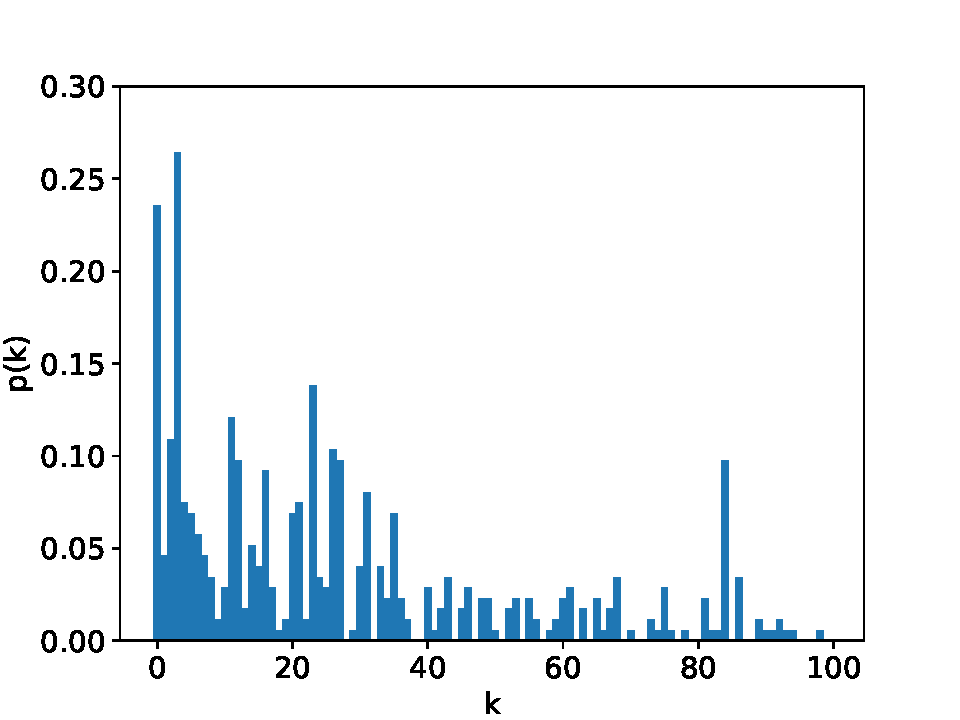
\includegraphics[width=0.6\textwidth]{graphs/survey_distribution_without_the_easy.pdf}
    % \caption{Performed on seven tasks, which did not contain the target person in the grid}
    % \label{fig:survey_all}
    % \end{subfigure}
    % \begin{subfigure}[b]{0.48\textwidth}
    %  \centering
    %  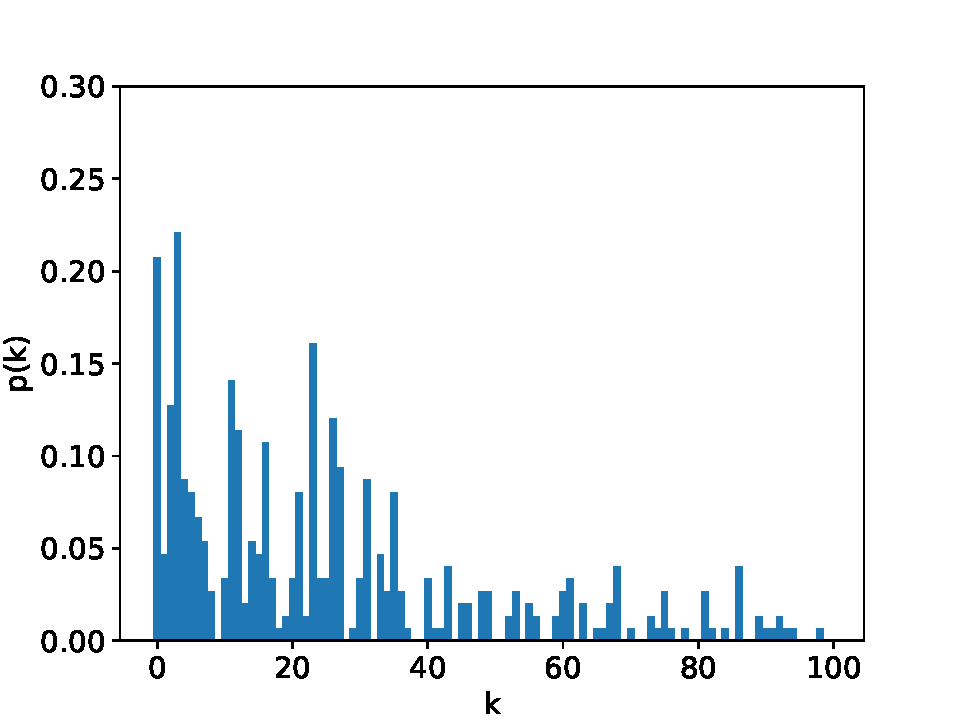
\includegraphics[width=\textwidth]{graphs/survey_distribution_childless.pdf}
    %  \caption{Performed on six tasks, extracting the task involving a child}
    %  \label{fig:suvery_childless}
    % \end{subfigure}
    
    \caption{Collected statistic on how likely user selects $k$-th closest face to the target in the face grid. Ideally, if user had been fully coherent with the distances in the features space, $p(R) = 1$ on $\{0,1,2\}$, since the user selected exactly 3 faces, and $p(R) = 0$ for all other $R$.}
    \label{fig:survey_distribution}
\end{figure}


\begin{figure}
    \centering
    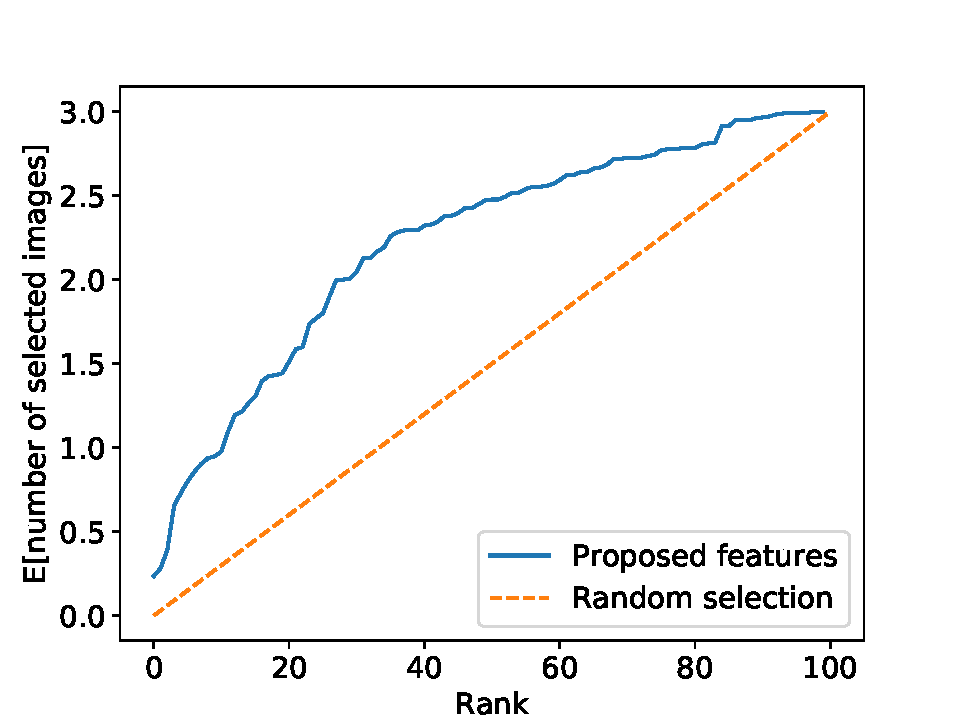
\includegraphics[width=0.8\linewidth]{graphs/survey_cumsum_without_the_easy.pdf}
    \caption{Expected value of the number of images selected up to a given rank.}
    \label{fig:random_selection_faces}
\end{figure}

\section{Building a traversal scheme}

In the previous sections, we extracted and encoded faces. In the case study, we investigated the feature space for the correspondence to the human annotations. Here we propose a solution of organizing faces into a multilevel view. 

As we discussed in \autoref{ch:related_work}, a common solution for the traversal system is a 2D grid.  In the 2D grid, a user can navigate using the following commands: move left, right, up, and down.


% This usually allows users navigation queries, as left, right, top, bottom. We call a set of images, which is visible at a particular step a \emph{display}. The display may contain tens to hundreds of images at once, depending on multiple factors, e.g., a user's screen size and the size of the displayed image.

Since most of the time, we want to browse more than a hundred images, it becomes inconvenient to preview dataset only in one layer. Therefore, we build a simple multilevel structure to ease the navigation.

\subsection{Tree-based structure}

Our goal is to organize a dataset of images $D$ to allow easy navigation. Let us assume that the dataset can be organized into a grid of size $N\times M$. We leave the choice of specific dimensions to the user. We prefer a square setting, although it is not required. In case that the size of the dataset $|D|$ is not square of any number, we recommend adding a placeholder images.

We organize (so far in a non-specific way) the items from the dataset into a chosen 2D grid. This is the base layer for the tree structure, we denote this grid as $L_0$. The layer has dimensions $L_{0, h}\times L_{0, w}$. Based on this layer, we create the next layer as only a subset of this layer. Firstly, we select $k$, which represents the sampling size factor. It means that every $k^2$-th image is selected as a representant to the next layer. The overview of the structure is shown in figure \ref{fig:tree_structure}. 

The layer $L_{i+1}$ has $1/k$ of the size in both axis of the $L_i$, more specifically, if the $L_i$ is of the dimensions $L_{i,h} \times L_{i,w}$, the layer $L_{i+1}$ has following dimensions:

$$
    L_{i+1, h} = \ceil*{L_{i, h} / k}
$$

$$
    L_{i+1, w} = \ceil*{L_{i, w} / k}
$$


The item on the position $m, n$ in the $L_{i+1}$ is replicated from the layer $L_i$ as follows:
$$
    L_{i+1, m, n} = L_{i, mk, nk} 
$$

We continue reducing the size of the layers until the layer will fit into a single display.

In this structure, we support six types of navigation: left, right, down, up, in and out. In and out represent operations of traversing between the layers and other directional commands allow navigation  within the layer. 

\begin{figure}
    \centering
    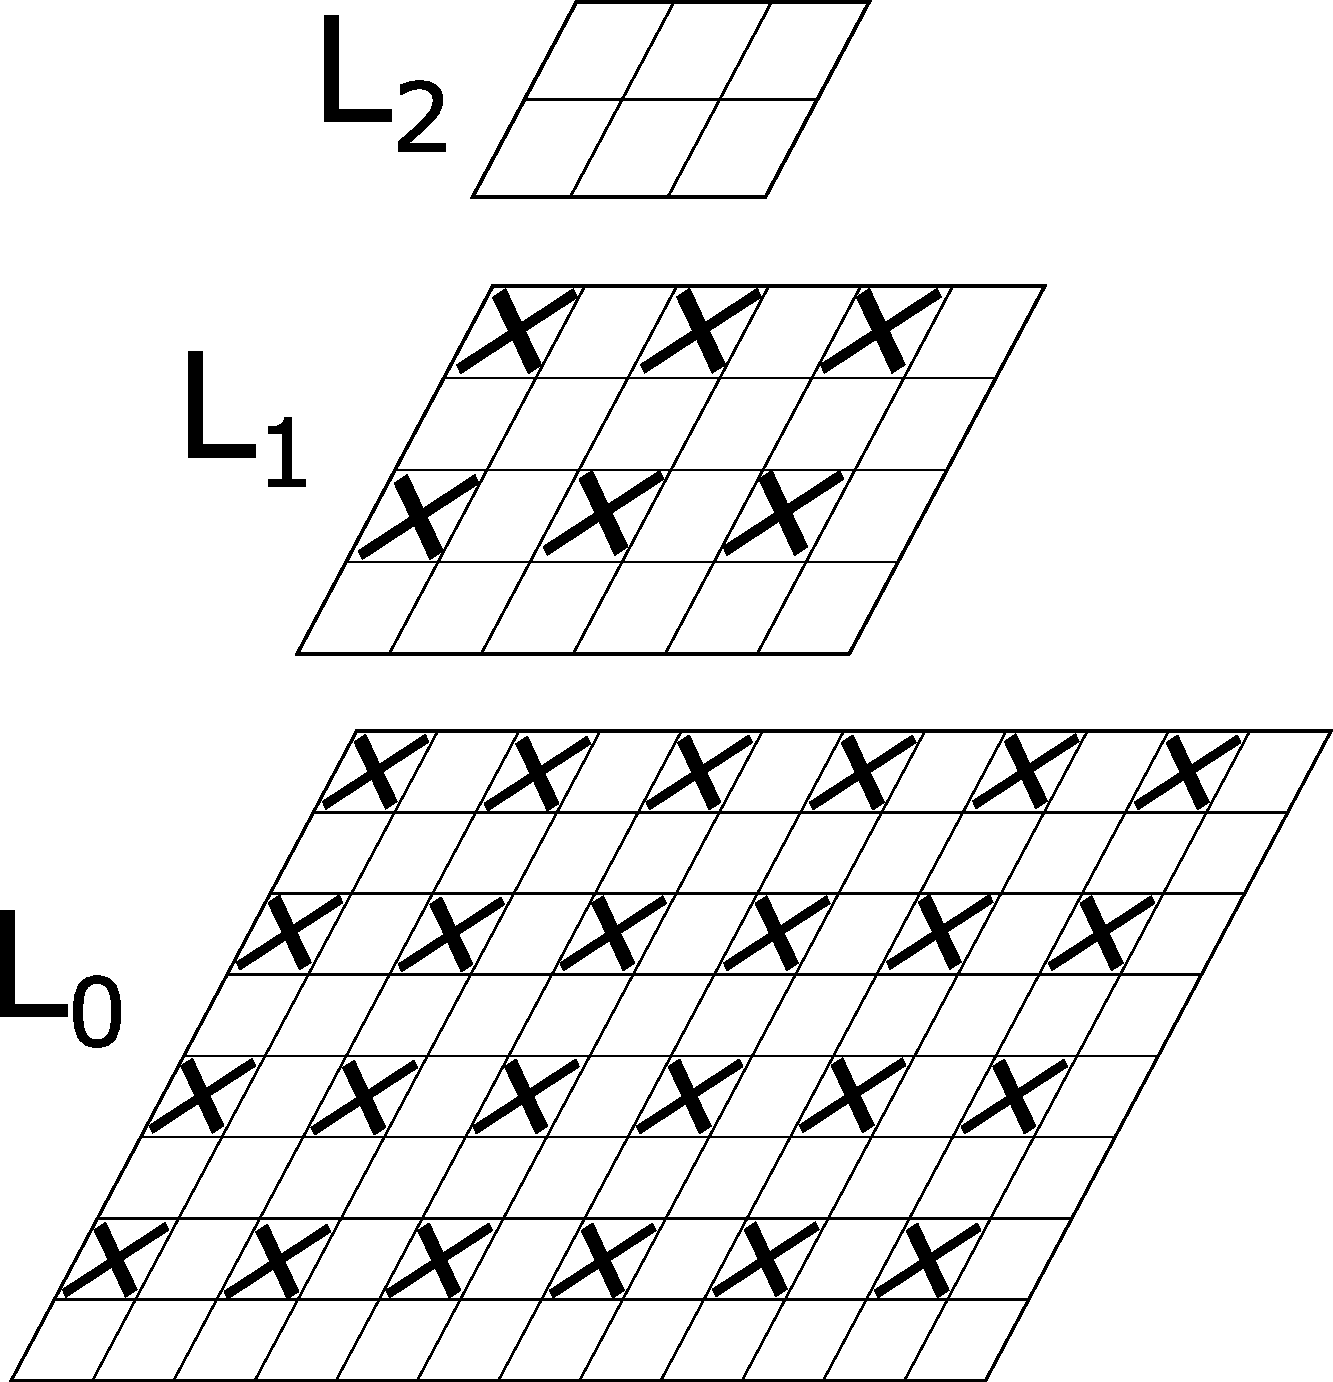
\includegraphics[width=0.3\linewidth]{img/tree-structure.pdf}
    \caption{A preview of the tree-based structure with $k = 2$ for previewing images. The marked items are selected for the layer above as representans.}
    \label{fig:tree_structure}
\end{figure}

\subsection{Bottom Layer -- Self-organizing map}

In the bottom layer, we would like to make use of the face encodings. As we reviewed in \autoref{ch:related_work}, Self-organizing maps showed a promising way to project high-dimensional data onto the 2D grid. We train a self-organizing map on our dataset of face encodings. For our particular dataset, we train a network of size $50\times 50$. This offers us 2500 neurons, having more neurons than there are faces in the dataset.

To train a SOM, we use a MiniSom framework \citep{vettigli2013minisom}. We use the default setting for the SOM, a gaussian neighborhood function with an asymptotic decay for the parameters. This setting showed the best results after visual inspection. We train the SOM for 200\,000 iterations, i.e., each example was seen on average 100 times during the training. Since the training of the SOM highly depends on the random initialization, we first run the same settings for ten different seeds for 30 000 iterations. Based on the results, we selected a seed with the lowest quantization error (refer to \autoref{s:som}). We reran the training with the best seed and trained for 200\,000 iterations.

\begin{figure}
    \centering
    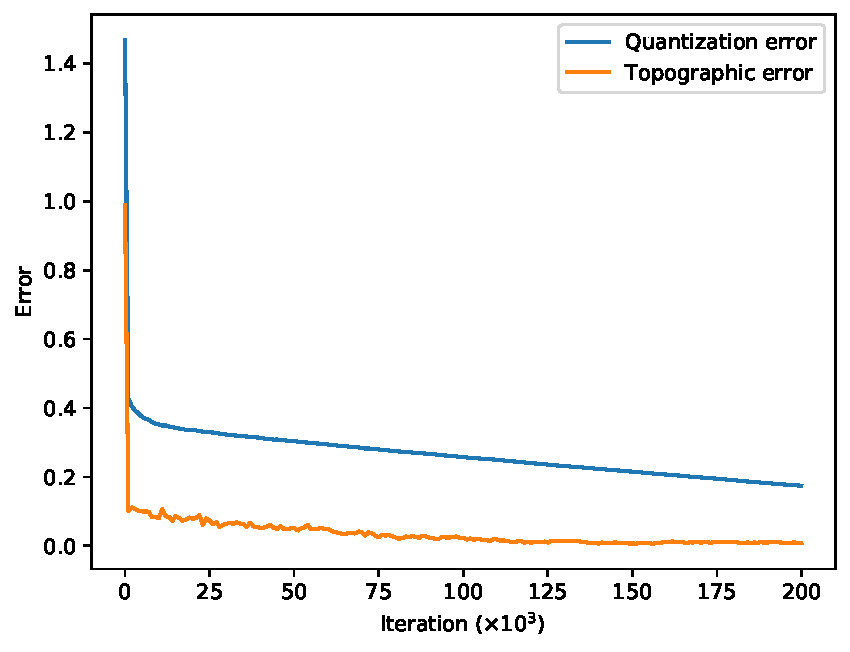
\includegraphics[width=0.8\linewidth]{graphs/som_errors.pdf}
    \caption{Training $50\times50$ SOM, 200 000 iterations.}
    \label{fig:som_training}
\end{figure}

The training errors are shown in figure \ref{fig:som_training}. We can observe that topographic error is at this stage stable. Even though the quantization error has not converged yet, at this stage, we did not achieve any improvements by our visual inspection.

Then we built the bottom layer for our traversal structure based on the trained SOM. This SOM represents our grid. For each neuron in the SOM, we assign a face whose encoding is closest to the given neuron's weight vector. We refer to this face as a representative of the given neuron.
Note that this way of selecting representatives does not avoid duplicates (i.e., assigning the same face to multiple neurons). 

We explored the assignments, and these are the observations we made: 345 faces out of original 2047 is not assigned to any of the neurons. However, only 22 out of these 345 faces have the distance to the closest face which is assigned to a neuron, higher than 0.45. In the original study, the authors of the model suggest considering encodings closer than 0.6 to be of the same person. As our investigation of the dataset in the figure \ref{fig:closest_faces} shows, threshold 0.45 is strict for assigning the same person. Therefore, we expect that those 323 faces missing represent a person, which is already among the representants. The maximum distance for the excluded 22 faces is 0.56, which is still below the initially proposed threshold for assigning the same person. Nevertheless, we verified that all of these faces, which are not selected as representants to any of the neurons of the \acrshort{som}, are still accessible from the structure by an additional utility that shows the most similar faces to a given face. We discuss this utility in the next section.

\subsection{Accessing the most similar faces}

We enhance the tree-structure to support displaying the most similar faces to a given face. A user can click on any of the displayed faces. Images, which contain a face considering to be the same person (threshold 0.6), are then displayed. This is helpful to find the exact target image when the user finds the same person on the map. This also provides a way to learn for the user. The user can display close faces, and investigate the characteristics by which faces are grouped by. Based on this, the user can utilize information about the structure to perform the face search faster in the next searches.

\section{Summary}

Our experiments suggest that the space of encodings contains some information on the face similarity. We propose a multilevel structure to explore a dataset of faces. In this structure, we support navigational commands that allow users to navigate within a layer (move left, right, up, and down) as well as traverse between the layers. Lower layers contain more faces, while upper layers offer a greater variety of the displayed faces.

We created the bottom layer with the help of a self-organizing map. We assigned each neuron its closest representative from the dataset. To provide users with additional insight into the data, we also support a search for closest faces to any given face in the traversal structure.

In the last section, we present a preliminary evaluation. More thorough evaluations, with more participants, would be needed to limit the user's memory and other factors. This would require different participants searching the datasets using different approaches and evaluating the time needed to find a face. Even though we do not provide such a complex study, we include the results of two respondents searching for ten faces using two different approaches.

\section{Preliminary evaluation}

In this section, we present a preliminary evaluation of the proposed navigational system. The goal of this chapter was to propose an exploration method over the dataset of faces. Therefore, we evaluate it by conducting an experiment with a user.

The task for the user is to find a target image in the dataset. As our baseline, we construct a grid of the faces, sorted by their original videos. Therefore, multiple images of one person are grouped together since they come from the same video. For searching in this grid, a user can only scroll up and down. We then test this approach against our traversal structure. The hypothesis we aim to prove is that our solution decreases the average time needed to find the target face compared to the search in random dataset.

For our experiment, we use ten randomly selected target images, which include faces. For each of them, we let the user search for the face in the dataset. Respondent A firstly searches for the faces in the baseline approach, then using the traversal structure. Respondent B searches in the opposite order, firstly they work with the traversal structure, and then with the baseline.

We measured the time required to successfully find the target image. We set the limit for this task to ten minutes. We obtained 20 measurements per approach. Respondent A was unable to retrieve a ``face 4'' within the time limit using either of the search approaches. These attempts were considered as 10 minutes of searching for the purposes of the evaluation. Respondent B successfully retrieved target images an all tasks.

Based on the experiment, we present results in graph \ref{fig:search_time}. In the case of both respondents, the median of the time required to solve the task was lower for the traversal search compared to the linear search. We also note that in terms of the average, we do not see any improvement.

% By the results, the traversal system did not performed significantly better, nor worse compared to the linear search. The traversal approach may still present a desired solution, when it comes to larger datasets. In such large datasets it may be impossible to go through all presented faces, one by one. The traversal search have an advantage of the interactive environment, where faces from several videos can be visually evaluated at once.

\begin{figure}
    \centering
    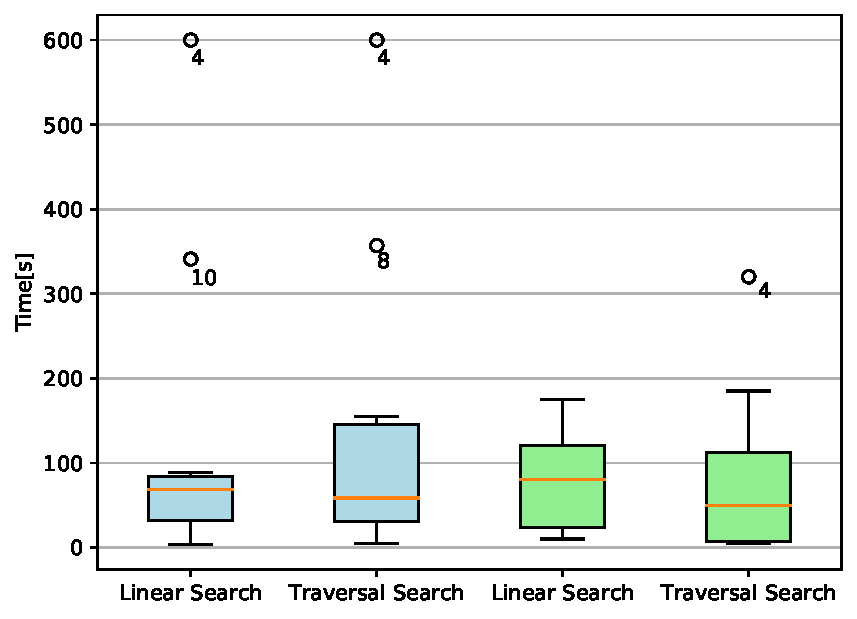
\includegraphics[width=0.7\linewidth]{graphs/face_search_time.pdf}
    \caption{Comparison of the time required to find a target image. Light blue belongs to the respondent A, light green to respondent B. The outliers are identified by the index of the task.}
    \label{fig:search_time}
\end{figure}